%% Contoh tesis GayaUKM dalam Bahasa Melayu
\documentclass[bahasam,nohyphen]{../../packages/GayaUKM}
\usepackage{../../packages/common}
% your thesis title (English)
\newcommand{\mytitle}{The Amazing Thesis that Would Blow \\ Your Frogging Mind}
% Your thesis title (bahasa)
\newcommand{\mytitlems}{Tesis yang Mengagumkan sehingga Menletupkan \\ kepada Otak Kau}
% your name
\newcommand{\myauthor}{Chin Chong Chang}
% your matric ID
\newcommand{\myauthorid}{P88888}
% faculty (English)
\newcommand{\myfaculty}{Faculty of Science and Technology}
% faculty (bahasa)
\newcommand{\myfacultyms}{Fakulti Sains dan Teknology}
% submission data
\newcommand{\mysubmissiondate}{\today}
% year
\newcommand{\mysubmissionyear}{2022}
% degree (English)
\newcommand{\mydegreetype}{Doctor of Philosophy}
% degree (bahasa)
\newcommand{\mydegreetypems}{Doktor Falsafah}
% campus
\campus{Bangi}


\title{\mytitlems}
\author{\myauthor}
\authorid{\myauthorid}
\faculty{\myfacultyms}
\submissiondate{\mysubmissiondate}
\submissionyear{\mysubmissionyear}
\degreetype{\mydegreetype}
\campus{Bangi} %% Assuming Malaysian cities are spelt the same way in English and Malay   

%% If you find the boxes around hyperlinks distracting
\hypersetup{colorlinks,allcolors=black}

\begin{document}

%% Cover page
\makecoverpage

%% Re-specify your title with different manual line breaks for the
%% title page, if necessary
\title{\mytitlems}
\maketitlepage

\frontmatter
\declaration

% penghargaan dari penghargaan.tex
\begin{acknowledgements}
Terima kasih kepada sekian yang menawarkan bantuan.
\end{acknowledgements}

% abstrak dlm Bahasa Melayu dari abstrak-ms.tex
\begin{msAbstract}
Inilah abstrak dalam Bahasa Melayu. Data korpus merupakan data bahasa
Melayu yang datangnya dalam dua bentuk sumber, iaitu bentuk tulisan
dan bentuk lisan. Bentuk tulisan seperti buku, majalah, surat khabar,
makalah, monograf, dokumen, kertas kerja, efemeral, puisi, drama,
kad bahan, surat, risalah dan sebagainya. Sementara bentuk lisan yang
ditranskripsikan seperti ucapan, wawancara, temu bual, perbualan dan
sebagainya dalam pelbagai bentuk rakaman.
\end{msAbstract}


% abstrak dlm Bahasa Inggeris dari abstract-en.tex
% Tajuk tesis dalam Bahasa Inggeris perlu diberikan.
\begin{enAbstract}[<Your English Title here>]
This is the English abstract. Auto single-line spacing. Jelly dessert sesame snaps. Oat cake jelly oat cake gingerbread sweet roll apple pie muffin sesame snaps. Dragée icing carrot cake faworki tart chocolate cake. Cookie apple pie chupa chups tootsie roll sweet roll toffee chocolate bar gummies gummi bears. Apple pie lollipop candy canes jujubes caramels. Soufflé powder liquorice fruitcake. Tiramisu fruitcake candy canes jelly beans muffin chupa chups bonbon. Donut sugar plum fruitcake liquorice chocolate pastry lollipop chocolate bar cookie. Jelly-o donut marshmallow chupa chups danish. Sugar plum pudding sweet roll muffin applicake biscuit tart fruitcake wafer. Pudding croissant carrot cake tiramisu candy canes. Powder powder jelly-o. Pie croissant cake chocolate cake carrot cake sweet apple pie sweet roll donut.
\end{enAbstract}


\tableofcontents\clearpage
\listoffigures\clearpage
\listoftables\clearpage

% Senari simbol dll boleh disediakan seperti
% dalam senaraisimbol.tex
\chapter{List of Symbols}

%% If your list of symbols/abbreviations are longer than a page, use a
%% longtable or supertabular instead e.g.
%% \begin{longtable}{l@\hspace{...}p{...}}
%% This will require \usepackage{longtable} or \usepackage{supertabular}
%% per your preference

\begin{center}
\doublespacing
\begin{longtable}{l@{\hspace{3em}}p{.6\textwidth}}
$b, c$ & constants\\
$C_f$ & local friction coefficient\\
\end{longtable}
\end{center}



\mainmatter
% Setiap satu bab dari fail berasingan
\chapter{Pengenalan}
\label{bab:pengenalan}

\section{Apakah Lorem Ipsum?}
\label{sec:apadia}

Lorem Ipsum adalah contoh teks atau dummy dalam industri percetakan dan penataan huruf atau typesetting. Lorem Ipsum telah menjadi standar contoh teks sejak tahun 1500an, saat seorang tukang cetak yang tidak dikenal mengambil sebuah kumpulan teks dan mengacaknya untuk menjadi sebuah buku contoh huruf \cite{banerjee:pedersen:2003}. Ia tidak hanya bertahan selama 5 abad, tapi juga telah beralih ke penataan huruf elektronik, tanpa ada perubahan apapun. Ia mulai dipopulerkan pada tahun 1960 dengan diluncurkannya lembaran-lembaran Letraset yang menggunakan kalimat-kalimat dari Lorem Ipsum, dan seiring munculnya perangkat lunak Desktop Publishing seperti Aldus PageMaker juga memiliki versi Lorem Ipsum \cite{berment:phd:2004}.



\section{Dari Mana Asalnya?}
\label{sec:asal}

\begin{equation}
C_p = \frac{P - P_\infty}{\frac{1}{2} \rho {U_\infty}^2}
 = 1 - \left( \frac{U_1}{U_\infty} \right)^2,
\end{equation}

Tidak seperti anggapan banyak orang, Lorem Ipsum bukanlah teks-teks yang diacak. Ia berakar dari sebuah naskah sastra latin klasik dari era 45 sebelum masehi, hingga bisa dipastikan usianya telah mencapai lebih dari 2000 tahun. Richard McClintock, seorang professor Bahasa Latin dari Hampden-Sidney College di Virginia, mencoba mencari makna salah satu kata latin yang dianggap paling tidak jelas, yakni consectetur, yang diambil dari salah satu bagian Lorem Ipsum. Setelah ia mencari maknanya di di literatur klasik, ia mendapatkan sebuah sumber yang tidak bisa diragukan. Lorem Ipsum berasal dari bagian 1.10.32 dan 1.10.33 dari naskah ``de Finibus Bonorum et Malorum'' (Sisi Ekstrim dari Kebaikan dan Kejahatan) karya Cicero, yang ditulis pada tahun 45 sebelum masehi \cite{azarova:etal:2002,budanitsky:hirst:2006}. Buku ini adalah risalah dari teori etika yang sangat terkenal pada masa Renaissance. Baris pertama dari Lorem Ipsum, ``Lorem ipsum dolor sit amet\ldots'', berasal dari sebuah baris di bagian 1.10.32.

Bagian standar dari teks Lorem Ipsum yang digunakan sejak tahun 1500an kini di reproduksi kembali di bawah ini untuk mereka yang tertarik. Bagian 1.10.32 dan 1.10.33 dari "de Finibus Bonorum et Malorum" karya Cicero juga di reproduksi persis seperti bentuk aslinya, diikuti oleh versi bahasa Inggris yang berasal dari terjemahan tahun 1914 oleh H. Rackham.

\begin{equation}
-\frac{(x_0 - \mu)^2}{2 \sigma^2} = -\ln 2
\end{equation}


\section{Contoh}
\label{sec:contol}

Perenggan awal Lorem Ipsum seperti di bawah.

\subsection{Perenggan Pertama}

Lorem ipsum dolor sit amet, consectetur adipiscing elit. Donec posuere, neque quis feugiat egestas, quam sapien dictum justo, eu vulputate nunc metus sed dui. Integer molestie leo quis libero facilisis, dictum pretium quam ornare. Vestibulum ante ipsum primis in faucibus orci luctus et ultrices posuere cubilia Curae; Vivamus luctus rutrum magna non convallis. Praesent vestibulum consequat eros, et fringilla nisi suscipit id. Nam vulputate justo dui, eu rutrum est accumsan ut. Sed molestie erat vitae mi blandit, in volutpat urna lobortis. Vestibulum mollis rutrum gravida. Fusce dolor nulla, condimentum vel pretium ut, venenatis eget leo. Ut semper placerat mauris, ut tempus est tempor vel. Interdum et malesuada fames ac ante ipsum primis in faucibus. In vitae feugiat diam. Pellentesque accumsan consequat turpis aliquam elementum.


\subsection{Dua Perenggan Seterusnya}

Vivamus dignissim arcu nunc, non aliquam sem porta vitae. Sed sodales accumsan dui sit amet egestas. Maecenas rhoncus a erat eget accumsan.

\begin{table}[hbt!]\centering
\caption{Bilangan permata}

\begin{tabular}{l c}
\hline
Jenis & Bilangan \\\hline
Nilam & 6\\
Berlian & 23\\
Emas & 56\\
Perak & 235\\
Gangsa & 324\\\hline
\end{tabular}
\end{table}

\begin{itemize}
\item Etiam vitae pulvinar metus, sed fringilla orci.
\item Duis dapibus dolor risus, non ultrices enim porta sit amet.
\item Ut eu libero augue.
\end{itemize}

Nulla ipsum augue, feugiat ac laoreet quis, pretium ut magna. Class aptent taciti sociosqu ad litora torquent per conubia nostra, per inceptos himenaeos. Integer blandit placerat dictum.

\begin{figure}[hbt!]\centering

\includegraphics[width=.5\textwidth]{green}
\caption{Contoh rajah}
\end{figure}

Sed dolor justo, scelerisque sed rutrum quis, porttitor a mauris. Cras non auctor felis, rutrum fringilla risus. Integer at convallis erat, sit amet luctus turpis. Duis sed rutrum eros, quis tempus risus. Etiam pellentesque nisi odio, eget dignissim eros ultrices et. Aliquam leo massa, fermentum vel odio sed, ullamcorper molestie lorem. Integer lorem felis, adipiscing sit amet interdum eget, auctor at lorem. Aliquam ultricies tortor eu nibh facilisis tincidunt.


\subsubsection{Sedikit Catatan}

Duis sed rutrum eros, quis tempus risus. Etiam pellentesque nisi odio, eget dignissim eros ultrices et. Aliquam leo massa, fermentum vel odio sed, ullamcorper molestie lorem.

\subsubsection{Selanjutnya}
Duis sed rutrum eros, quis tempus risus. Etiam pellentesque nisi odio, eget dignissim eros ultrices et. Aliquam leo massa, fermentum vel odio sed, ullamcorper molestie lorem.


\section{Ringkasan}
Nulla ipsum augue, feugiat ac laoreet quis, pretium ut magna. Class aptent taciti sociosqu ad litora torquent per conubia nostra, per inceptos himenaeos. Integer blandit placerat dictum.

Sed dolor justo, scelerisque sed rutrum quis, porttitor a mauris. Cras non auctor felis, rutrum fringilla risus. Integer at convallis erat, sit amet luctus turpis. Duis sed rutrum eros, quis tempus risus. Etiam pellentesque nisi odio, eget dignissim eros ultrices et. Aliquam leo massa, fermentum vel odio sed, ullamcorper molestie lorem. Integer lorem felis, adipiscing sit amet interdum eget, auctor at lorem. Aliquam ultricies tortor eu nibh facilisis tincidunt.

\chapter{Latar Belakang}

Lorem ipsum dolor sit amet, consectetur adipiscing elit. Donec posuere, neque quis feugiat egestas, quam sapien dictum justo, eu vulputate nunc metus sed dui. Integer molestie leo quis libero facilisis, dictum pretium quam ornare. Vestibulum ante ipsum primis in faucibus orci luctus et ultrices posuere cubilia Curae; Vivamus luctus rutrum magna non convallis. Praesent vestibulum consequat eros, et fringilla nisi suscipit id. Nam vulputate justo dui, eu rutrum est accumsan ut. Sed molestie erat vitae mi blandit, in volutpat urna lobortis. Vestibulum mollis rutrum gravida. Fusce dolor nulla, condimentum vel pretium ut, venenatis eget leo. Ut semper placerat mauris, ut tempus est tempor vel. Interdum et malesuada fames ac ante ipsum primis in faucibus. In vitae feugiat diam. Pellentesque accumsan consequat turpis aliquam elementum.
\chapter{Golden Ratio}

In mathematics and the arts, two quantities are in the golden ratio if their ratio is the same as the ratio of their sum to the larger of the two quantities, i.e.~their maximum. The figure on the right illustrates the geometric relationship. Expressed algebraically, for quantities $a$ and $b$ with $a > b$,
\begin{equation}
 \frac{a+b}{a} = \frac{a}{b} \ \stackrel{\text{def}}{=}\ \varphi,
\end{equation}
where the Greek letter $\varphi$ represents the golden ratio. Its value is:
\begin{equation}
\varphi = \frac{1+\sqrt{5}}{2} = 1.61803\,39887\ldots.
\end{equation}

\section{History}

Ancient Greek mathematicians first studied what we now call the golden ratio because of its frequent appearance in geometry. The division of a line into ``extreme and mean ratio'' (the golden section) is important in the geometry of regular pentagrams and pentagons. Euclid's Elements  provides the first known written definition of what is now called the golden ratio: ``A straight line is said to have been cut in extreme and mean ratio when, as the whole line is to the greater segment, so is the greater to the less.'' Euclid explains a construction for cutting (sectioning) a line ``in extreme and mean ratio'', i.e., the golden ratio. (See Figure~\ref{fig:line:golden}.) Throughout the Elements, several propositions (theorems in modern terminology) and their proofs employ the golden ratio.

\begin{figure}[hbt!]\centering
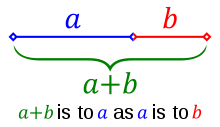
\includegraphics[width=.3\textwidth]{220px-Golden-ratio-line}
\caption{Line segments in the golden ratio}
\label{fig:line:golden}
\end{figure}

\begin{figure}[hbt!]\centering
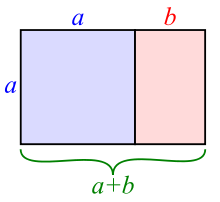
\includegraphics[width=.3\textwidth]{SimilarGoldenRectangles}
\caption{Golden rectangles}
\end{figure}



\section{Calculation}
Two quantities $a$ and $b$ are said to be in the golden ratio $\varphi$ if:
\begin{equation}
 \frac{a+b}{a} = \frac{a}{b} = \varphi.
\end{equation}

One method for finding the value of $\varphi$ is to start with the left fraction. Through simplifying the fraction and substituting in $\frac{b}{a} = \frac{1}{\varphi}$,
\begin{equation}
\frac{a+b}{a} = 1 + \frac{b}{a} = 1 + \frac{1}{\varphi},
\end{equation}

By definition, it is shown that
\begin{equation}
 1 + \frac{1}{\varphi} = \varphi. 
\end{equation}
Multiplying by $\varphi$ gives
\begin{equation*}
\varphi + 1 = \varphi^2
\end{equation*}
which can be rearranged to
\begin{equation*}
{\varphi}^2 - \varphi - 1 = 0.
\end{equation*}
Using the quadratic formula, two solutions are obtained:
\begin{equation*}
\varphi = \frac{1 + \sqrt{5}}{2} = 1.61803\,39887\dots
\end{equation*}
and
\begin{equation*}
\varphi = \frac{1 - \sqrt{5}}{2} = -0.6180\,339887\dots
\end{equation*}
Because $\varphi$ is the ratio between positive quantities $\varphi$ is necessarily positive:
\begin{equation*}
\varphi = \frac{1 + \sqrt{5}}{2} = 1.61803\,39887\dots .
\end{equation*}

Different representations of the golden ratio are given in Table~\ref{tab:goldenratio}.

\begin{table}[hbt!]\centering
\caption{Number representations of the golden ratio}
\label{tab:goldenratio}

\begin{tabular}{|l|l|}
\hline
Form & Representation\\\hline
Binary & 1.1001111000110111011\ldots\\\hline
Decimal & 1.6180339887498948482\ldots\\\hline
Hexadecimal	& 1.9E3779B97F4A7C15F39\ldots\\\hline
Continued fraction & $1 + \cfrac{1}{1 + \cfrac{1}{1 + \cfrac{1}{1 + \cfrac{1}{1 + \ddots}}}}$\\[6ex]\hline
Algebraic form & $\displaystyle\frac{1 + \sqrt{5}}{2}$\\[2ex]\hline
Infinite series & $\displaystyle\frac{13}{8}+\sum_{n=0}^{\infty}\frac{(-1)^{(n+1)}(2n+1)!}{(n+2)!\,n!\,4^{(2n+3)}}$\\[2ex]\hline
\end{tabular}
\end{table}

\chapter{Fibonacci Numbers}

In mathematics, the Fibonacci numbers or Fibonacci series or Fibonacci sequence are the numbers in the following integer sequence:
%
\begin{equation*} % example of unnumbered equations
0, 1, 1, 2, 3,5,8,13,21,34,55,89,144,\ldots
\end{equation*}

By definition, the first two numbers in the Fibonacci sequence are 0 and 1, and each subsequent number is the sum of the previous two. In mathematical terms, the sequence $F_n$ of Fibonacci numbers is defined by the recurrence relation
%
\begin{equation}
F_n = F_{n-1} + F_{n-2},
\end{equation}
%
with seed values
%
\begin{equation}
F_0 = 0, F_1 = 1.
\end{equation}

The Fibonacci sequence is named after Leonardo Fibonacci. His 1202 book Liber Abaci introduced the sequence to Western European mathematics, although the sequence had been described earlier in Indian mathematics. \cite{Goonatilake:1998} By modern convention, the sequence begins either with $F_0 = 0$ or with $F_1 = 1$. The Liber Abaci began the sequence with $F_1 = 1$, without an initial 0.


\section{Origins}

The Fibonacci sequence appears in Indian mathematics, in connection with Sanskrit prosody. \cite{Singh:1985} In the Sanskrit oral tradition, there was much emphasis on how long (L) syllables mix with the short (S), and counting the different patterns of L and S within a given fixed length results in the Fibonacci numbers; the number of patterns that are m short syllables long is the Fibonacci number $F_{m + 1}$.
\citet{Goonatilake:1998} writes that the development of the Fibonacci sequence ``is attributed in part to Pingala (200 BC), later being associated with Virahanka (c.~700 AD), Gopala (c.~1135), and Hemachandra (c.~1150)''.

\begin{figure}[hbt!]
\centering
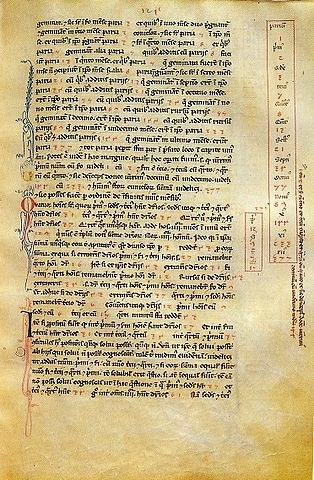
\includegraphics[width=.4\textwidth]{314px-Liber-abbaci-magliab-f124r}
\caption{A page of Fibonacci's Liber Abaci}
\source{Heinz L\"{u}neburg, Leonardi Pisani Liber Abaci oder Lesevergn\"{u}gen eines Mathematikers}
\end{figure}

\section{List of Fibonacci Numbers}

The first 11 Fibonacci numbers $F_n$ for $n = 0, 1, 2, \ldots, 10$ are:

\begin{table}[hbt!]\centering
\caption{First 11 Fibonacci Numbers for $n=0,1,\ldots$}
\begin{tabular}{|c|c|c|c|c|c|c|c|c|c|c|}
\hline
$F_0$ & $F_1$ & $F_2$ & $F_3$ & $F_4$ & $F_5$ & $F_6$ & $F_7$ & $F_8$ & $F_9$ & $F_{10}$\\
\hline
0 & 1 & 1 & 2 & 3 & 5 & 8 & 13 & 21 & 34 & 55 \\
\hline
\end{tabular}
\end{table}

The sequence can also be extended to negative index n using the re-arranged recurrence relation
%
\begin{equation}
F_{n-2} = F_n - F_{n-1},
\end{equation}
%
which yields the sequence of ``negafibonacci'' numbers satisfying
%
\begin{equation}
F_{-n} = (-1)^{n+1} F_n.
\end{equation}
%
Thus the bidirectional sequence is
\begin{table}[hbt!]\centering
\caption{Bidirectional Fibonacci Numbers sequence}
\begin{tabular}{|c|c|c|c|c|c|c|c|c|c|c|}
\hline
$F_{-5}$ & $F_{-4}$ & $F_{-3}$ & $F_{-2}$ & $F_{-1}$ & $F_0$ & $F_1$ & $F_2$ & $F_3$ & $F_4$ & $F_5$ \\\hline
5 & $-3$ & 2 & $-1$ & 1 & 0 & 1 & 1 & 2 & 3 & 5\\\hline
\end{tabular}
\end{table}

\citet{Rohl:1989} gives an account of how Fibonacci numbers can be computed efficiently.

\section{Applications}

\subsection{In Computation}

Fibonacci numbers have wide applications in mathematics as well as computer science:

\begin{itemize}
\item The Fibonacci numbers are important in the computational run-time analysis of Euclid's algorithm to determine the greatest common divisor of two integers: the worst case input for this algorithm is a pair of consecutive Fibonacci numbers.

\item Yuri Matiyasevich was able to show that the Fibonacci numbers can be defined by a Diophantine equation, which led to his original solution of Hilbert's tenth problem.

\item The Fibonacci numbers are also an example of a complete sequence. This means that every positive integer can be written as a sum of Fibonacci numbers, where any one number is used once at most.

\item Moreover, every positive integer can be written in a unique way as the sum of one or more distinct Fibonacci numbers in such a way that the sum does not include any two consecutive Fibonacci numbers. This is known as Zeckendorf's theorem, and a sum of Fibonacci numbers that satisfies these conditions is called a Zeckendorf representation. The Zeckendorf representation of a number can be used to derive its Fibonacci coding.

\item Fibonacci numbers are used by some pseudorandom number generators.

\item Fibonacci numbers are used in a polyphase version of the merge sort algorithm in which an unsorted list is divided into two lists whose lengths correspond to sequential Fibonacci numbers -- by dividing the list so that the two parts have lengths in the approximate proportion $\varphi$. A tape-drive implementation of the polyphase merge sort was described in The Art of Computer Programming.

\item Fibonacci numbers arise in the analysis of the Fibonacci heap data structure.

\item The Fibonacci cube is an undirected graph with a Fibonacci number of nodes that has been proposed as a network topology for parallel computing.

\item A one-dimensional optimization method, called the Fibonacci search technique, uses Fibonacci numbers.

\item The Fibonacci number series is used for optional lossy compression in the IFF 8SVX audio file format used on Amiga computers. The number series compands the original audio wave similar to logarithmic methods such as $\mu$-law.

\item Since the conversion factor 1.609344 for miles to kilometers is close to the golden ratio (denoted $\varphi$), the decomposition of distance in miles into a sum of Fibonacci numbers becomes nearly the kilometer sum when the Fibonacci numbers are replaced by their successors. This method amounts to a radix 2 number register in golden ratio base $\varphi$ being shifted. To convert from kilometers to miles, shift the register down the Fibonacci sequence instead.
\end{itemize}


\subsection{In Nature}

Fibonacci sequences appear in biological settings, in two consecutive Fibonacci numbers, such as branching in trees, arrangement of leaves on a stem, the fruitlets of a pineapple, the flowering of artichoke, an uncurling fern and the arrangement of a pine cone, and the family tree of honeybees. However, numerous poorly substantiated claims of Fibonacci numbers or golden sections in nature are found in popular sources, e.g.,~relating to the breeding of rabbits in Fibonacci's own unrealistic example, the seeds on a sunflower, the spirals of shells, and the curve of waves.

A model for the pattern of florets in the head of a sunflower was proposed by H.~Vogel in 1979. \cite{Vogel:1979} This has the form
\begin{equation}
\theta = \frac{2\pi}{\phi^2} n,\  r = c \sqrt{n}
\end{equation}
where $n$ is the index number of the floret and $c$ is a constant scaling factor; the florets thus lie on Fermat's spiral.

\begin{figure}[hbt!]\centering
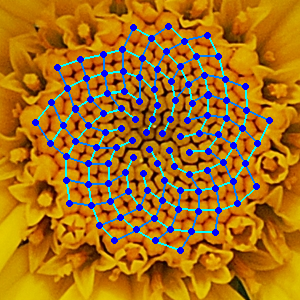
\includegraphics[width=.5\textwidth]{FibonacciChamomile}

\caption{Yellow Chamomile head}
\end{figure}


% rujukan tersenarai dlm refs.bib
\bibliography{../references}

\appendix
% Setiap satu bab apendiks dari fail berasingan
\chapter{Details}

Lorem ipsum dolor sit amet, consectetur adipiscing elit. Donec posuere, neque quis feugiat egestas, quam sapien dictum justo, eu vulputate nunc metus sed dui. Integer molestie leo quis libero facilisis, dictum pretium quam ornare. Vestibulum ante ipsum primis in faucibus orci luctus et ultrices posuere cubilia Curae; Vivamus luctus rutrum magna non convallis. Praesent vestibulum consequat eros, et fringilla nisi suscipit id. Nam vulputate justo dui, eu rutrum est accumsan ut. Sed molestie erat vitae mi blandit, in volutpat urna lobortis. Vestibulum mollis rutrum gravida. Fusce dolor nulla, condimentum vel pretium ut, venenatis eget leo. Ut semper placerat mauris, ut tempus est tempor vel. Interdum et malesuada fames ac ante ipsum primis in faucibus. In vitae feugiat diam. Pellentesque accumsan consequat turpis aliquam elementum.
\chapter{Software Code}

\begin{lstlisting}[language=Python, caption=Python example]
import numpy as np
    
def incmatrix(genl1,genl2):
    m = len(genl1)
    n = len(genl2)
    M = None #to become the incidence matrix
    VT = np.zeros((n*m,1), int)  #dummy variable
    
    #compute the bitwise xor matrix
    M1 = bitxormatrix(genl1)
    M2 = np.triu(bitxormatrix(genl2),1) 

    for i in range(m-1):
        for j in range(i+1, m):
            [r,c] = np.where(M2 == M1[i,j])
            for k in range(len(r)):
                VT[(i)*n + r[k]] = 1;
                VT[(i)*n + c[k]] = 1;
                VT[(j)*n + r[k]] = 1;
                VT[(j)*n + c[k]] = 1;
                
                if M is None:
                    M = np.copy(VT)
                else:
                    M = np.concatenate((M, VT), 1)
                
                VT = np.zeros((n*m,1), int)
    
    return M
\end{lstlisting}


\end{document}
